\documentclass{beamer}
\usepackage[english,russian]{babel}
\usepackage[utf8]{inputenc}
\usepackage{mathtext}
% Стиль презентации
\usetheme{Singapore}
\usecolortheme{default}

\begin{document}


\title{Моделирование процесса прокатки титанового прутка в пакете Deform 3D}  
\author{Ибрагимов Ринат, ОНФ ПМИ-34}
\date{УГАТУ, 2013}
% Создание заглавной страницы
\frame{\titlepage}
\frame{
 \frametitle{Содержание}
 \tableofcontents
Описание процесса моделирования прокатки титанового прутка в программе «Deform 3D» и анализ результатов с целью дальнейшего изучения изменения зернистости металла
} 
\begin{frame}{Постановка задачи}
Изучить систему конечно-элементного моделирования DEFORM-3D, предназначенную для анализа трёхмерного течения металла при различных процессах обработки металла давлением.
Пользуясь системой DEFORM смоделировать процесс прокатки титанового прутка метровой длины и оценить изменения произошедшие в его геометрии в результате процесса.
\end{frame}

\begin{frame}{Практическая часть}
В Пакете Deform 3D смоделирован механизм, состоящий из двух вращающихся валов и направляющей трубки, в которую будет помещаться пруток.

Валы вращаются таким образом, что протскивают пруток между собой, обжимая его, при этом расширяя и удлинняя.

Расстояние между валами равно пяти миллиметрам.
\end{frame}

\begin{frame}{Практическая часть}
\begin{figure}[h]
 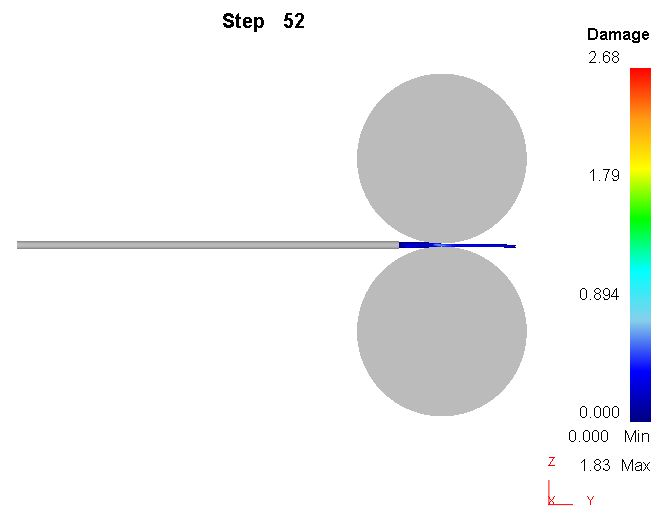
\includegraphics[width=3in]{img/step52.JPG}
 \footnotesize\caption{Вид установки в момент расчёта}
\end{figure}
\end{frame}

\begin{frame}{Практическая часть}
\begin{figure}[h]
 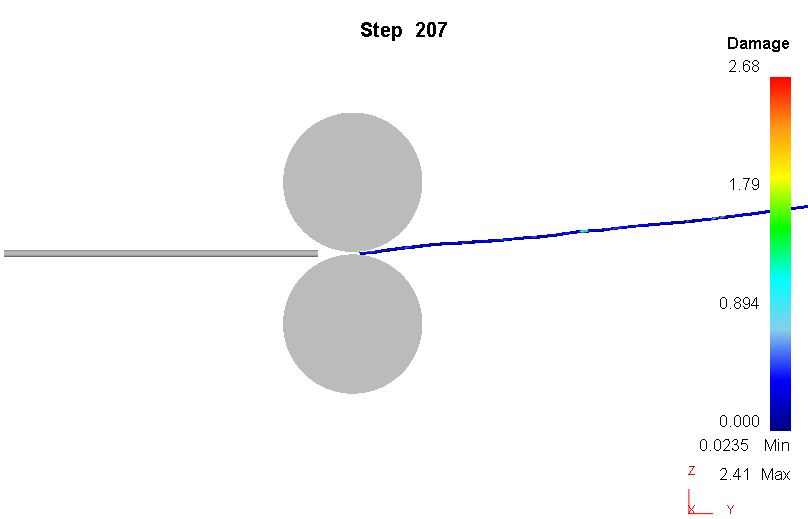
\includegraphics[width=3in]{img/step207.JPG}
 \footnotesize\caption{Вид установки в конце расчёта}
\end{figure}
\end{frame}

\begin{frame}{Практическая часть}
\begin{figure}[h]
 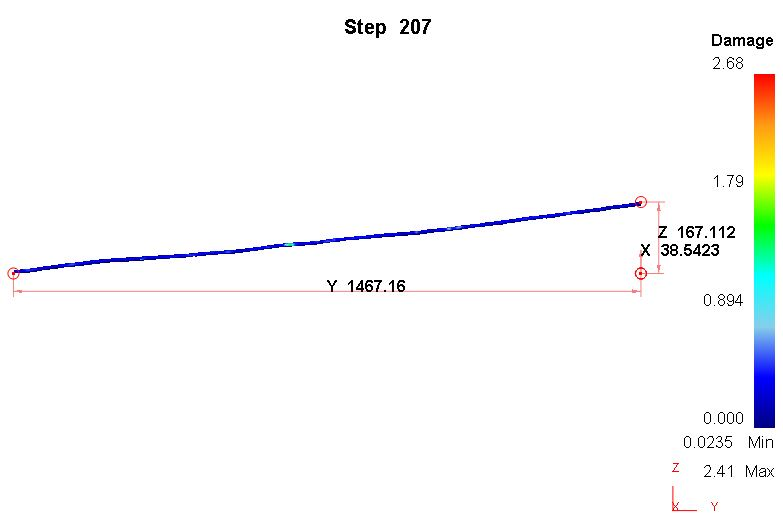
\includegraphics[width=3in]{img/step207_3.JPG}
 \footnotesize\caption{Вид прутка в конце расчёта}
\end{figure}
\end{frame}

\begin{frame}{Дополнительно}
В процессе выполнения работы таже были проверены другие материалы и температуры
\begin{figure}[h]
 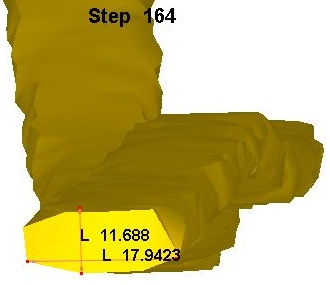
\includegraphics[width=3in]{img/164_2.JPG}
 \footnotesize\caption{Алюминиевый прут}
\end{figure}
\end{frame}

\begin{frame}{Заключение}
С помощью системы DEFORM-3D удалось смоделировать процесс прокатки титанового прута 1000x15мм, и оценить его деформации.
При сжатии до высоты в 7мм, происходит удлинение более чем в полтора раза, расширение приблизительно до 24мм, и изгибы, из-за которых, к сожалению, не удаётся точно измерить получившуюся геометрию средствами DEFORM.
\end{frame}

\begin{frame}{Список литературы}
В.С. Паршин, А.П. Карамышев, И.И. Некрасов, А.И. Пугин, А.А. Федулов
Учебное пособие под редакцией д-ра технических наук Ю.Б. Чечулина
Практическое руководство к программному компексу DEFORM-3D
Екатеринбург, УрФУ, 2010
\end{frame}

\begin{frame}{Спасибо за внимание!}
\vfill
\centering\LaTeX
\end{frame}

\end{document}